%
% section 3.3
%
\section{Πρωτόκολλα Ανεύρεσης και Απόδοσης Διευθύνσεων, Address Resolution Protocol (ARP) και Dynamic Host Configuration Protocol (DHCP)}

Όπως έχουμε δει μέχρι τώρα, το κάθε επίπεδο παραλαμβάνει τα δεδομένα από το αμέσως ανώτερο επίπεδο και προσθέτει σε αυτά τις δικές του διαχειριστικές πληροφορίες (τη δική του επικεφαλίδα) σε μια διαδικασία που έχουμε ονομάσει ενθυλάκωση. Σε κάθε επίπεδο τα δεδομένα περιέχουν όλες τις πληροφορίες και τις επικεφαλίδες των προηγούμενων επιπέδων ενώ προστίθεται και μια καινούρια. Σε κάποια επίπεδα επίσης μπορεί να γίνεται κατακερματισμός των δεδομένων σε μικρότερα κομμάτια (στο επίπεδο μεταφοράς αυτό το κάνει το TCP και στο επίπεδο δικτύου το IP). Σε κάθε επίπεδο επίσης η μονάδα δεδομένων έχει διαφορετικό όνομα: στο επίπεδο μεταφοράς, στο πρωτόκολλο TCP έχουμε τμήματα (segments), στο επίπεδο δικτύου με το πρωτόκολλο IP έχουμε πακέτα (packets) και στο επίπεδο ζεύξης δεδομένων (για δίκτυο Ethernet) έχουμε πλαίσια (frames). 


\begin{figure}[!ht]
  \centering
  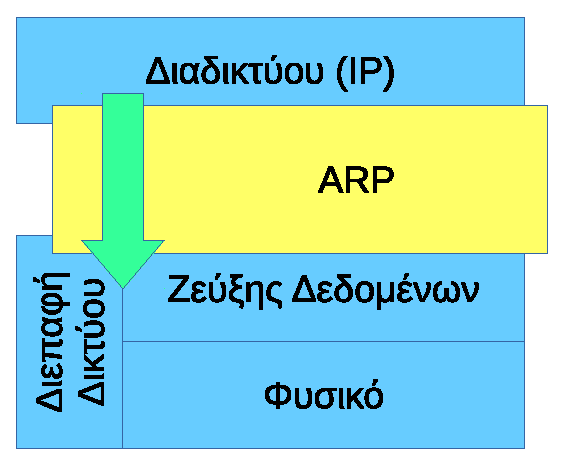
\includegraphics[width=0.65\textwidth]{images/chapter3/3-15}
  \caption {\textsl{Το Πρωτόκολλο ARP}}
  \label{3-15}
\end{figure}


Στο επίπεδο δικτύου προστίθενται οι λογικές διευθύνσεις (διευθύνσεις IP) και δημιουργούνται αυτοδύναμα πακέτα. Τα πακέτα αυτά θα πρέπει να προωθηθούν στο επίπεδο ζεύξης δεδομένων για να αποσταλούν στο φυσικό μέσο και να παραδοθούν. Το πρόβλημα είναι ότι το επίπεδο ζεύξης δεδομένων δεν γνωρίζει τίποτα για τις λογικές διευθύνσεις του επιπέδου δικτύου: γνωρίζει μόνο τις δικές του φυσικές (MAC) διευθύνσεις. Για να μπορέσει να παραδώσει τα δεδομένα, θα πρέπει να δημιουργήσει πλαίσια στα οποία οι επικεφαλίδες να περιέχουν τις φυσικές διευθύνσεις αποστολέα και παραλήπτη (θυμηθείτε το πλαίσιο Ethernet που είδαμε στο κεφάλαιο 2).

θα πρέπει με κάποιο τρόπο να μετατραπούν οι λογικές διευθύνσεις σε φυσικές. Τη μετατροπή αυτή την κάνει το \emph{πρωτόκολλο ARP}, το οποίο δρα σα συνδετικός κρίκος (σχήμα \ref{3-15}) μεταξύ του επιπέδου δικτύου και του επιπέδου ζεύξης δεδομένων.

\begin{inthebox}
\textbf{Σε ποιο επίπεδο είναι το πρωτόκολλο ARP;}

Το σχήμα του βιβλίου σας δείχνει το ARP ανάμεσα στα επίπεδα δικτύου και ζεύξης δεδομένων. Στο OSI συχνά αναφέρεται ως πρωτόκολλο επιπέδου 3 (Δικτύου) το οποίο ενθυλακώνεται σε πρωτόκολλα επιπέδου 2 (τα ερωτήματα και οι απαντήσεις ARP γίνονται μέσω πλαισίων). Ωστόσο το ARP δεν έχει σχεδιαστεί με βάση το μοντέλο OSI (το Ethernet προϋπάρχει του OSI) και έτσι η παραπάνω ταξινόμηση είναι κάπως αυθαίρετη. Είναι πιο σωστό να το θεωρήσουμε ως λειτουργία που βρίσκεται ενδιάμεσα στα δύο επίπεδα (cross layer function). Στο μοντέλο TCP/IP, τα χαρακτηριστικά του ARP το κατατάσσουν στο επίπεδο ζεύξης δεδομένων.\\
\end{inthebox}

Το \emph{ARP, Πρωτόκολλο Ανάλυσης Διευθύνσεων, Address Resolution Protocol}  αναλαμβάνει να απαντήσει σε ερωτήματα του τύπου ``Ποια είναι η φυσική (MAC) διεύθυνση του υπολογιστή με τη συγκεκριμένη διεύθυνση IP;'' 

Για να επιτελέσει το σκοπό του, το πρωτόκολλο ARP χρησιμοποιεί το \emph{ερώτημα ARP (ARP request)} με το οποίο απευθύνεται στο τοπικό δίκτυο Ethernet. Το ερώτημα αυτό γίνεται με ένα πλαίσιο εκπομπής: θυμηθείτε από το Ethernet ότι η φυσική διεύθυνση εκπομπής είναι άσοι και στα 48 ψηφία, ή στο δεκαεξαδικό FF:FF:FF:FF: FF:FF. Με αυτή τη διεύθυνση παραλήπτη, το ερώτημα θα ληφθεί από όλους τους κόμβους.

Κάθε κόμβος συγκρίνει την ζητούμενη IP με τη δική του και αν δεν συμπίπτει, απλά θα αγνοήσει το ερώτημα. Ο κόμβος όμως που διαθέτει τη συγκεκριμένη IP θα διαμορφώσει μια κατάλληλη \emph{απάντηση ARP (ARP Reply)} και θα την αποστείλει στον κόμβο που έκανε την ερώτηση.

Επειδή είναι χρονοβόρο (και προκαλεί και αυξημένη κίνηση στο δίκτυο) να γίνεται συνέχεια η ίδια ερώτηση σε κάθε μετάδοση, κάθε κόμβος αποθηκεύει τις απαντήσεις που λαμβάνει προσωρινά στην τοπική μνήμη, σε ένα πίνακα που ονομάζεται \emph{ARP Cache}. Πριν ένας κόμβος υποβάλλει ερώτημα στο δίκτυο, ελέγχει πρώτα από όλα τον τοπικό του πίνακα και αν υπάρχει αντίστοιχη καταχώριση την χρησιμοποιεί. Πρέπει να σημειώσουμε ότι κάθε κόμβος έχει δικό του πίνακα ARP με τις απαντήσεις στα ερωτήματα που έχει υποβάλλει ο ίδιος μέχρι στιγμής. Αν ένας κόμβος έχει περισσότερες από μια κάρτες δικτύου (για παράδειγμα αν είναι συνδεδεμένος με περισσότερα από ένα δίκτυα), υπάρχει ένας πίνακας ARP για κάθε κάρτα δικτύου. 

\begin{figure}[!ht]
  \centering
  \includegraphics[width=0.95\textwidth]{images/chapter3/3-10}
  \caption {\textsl{Εκτέλεση εντολής arp σε ένα UNIX σύστημα}}
  \label{3-10}
\end{figure}

Οι καταχωρίσεις στον πίνακα ARP είναι μπορεί να είναι \emph{στατικές ή δυναμικές}. Οι δυναμικές καταχωρίσεις είναι προσωρινές: μετά από κάποιο χρονικό διάστημα (από μερικά δευτερόλεπτα ως λίγα λεπτά συνήθως, το διάστημα μπορεί να ρυθμιστεί από το διαχειριστή του δικτύου) οι καταχωρίσεις λήγουν και το αντίστοιχο ερώτημα πρέπει να γίνει εκ νέου. Αντίθετα οι στατικές καταχωρίσεις έχουν μόνιμη ισχύ και δε λήγουν (παράδειγμα στατικής καταχώρισης είναι αυτή που αντιστοιχεί στην κάρτα δικτύου του ίδιου του μηχανήματος). Στο σχήμα \ref{3-10} βλέπουμε τον πίνακα ARP σε ένα μηχάνημα UNIX (FreeBSD). Η ένδειξη ``expires'' δείχνει σε πόσα δευτερόλεπτα λήγει κάθε καταχώριση του πίνακα. Μετά τη λήξη, θα πρέπει να δημιουργηθεί ξανά ερώτημα ARP για τη συγκεκριμένη διεύθυνση. Η μόνιμη (permanent) καταχώριση στον πίνακα αντιστοιχεί στο ίδιο το μηχάνημα που εκτελεί την εντολή.

Το πακέτο ARP που αντιστοιχεί στο ερώτημα ενθυλακώνεται σε ένα πλαίσιο Ethernet και έχει τη μορφή που φαίνεται στο σχήμα \ref{3-11}. 

\begin{figure}[!ht]
 \centering
 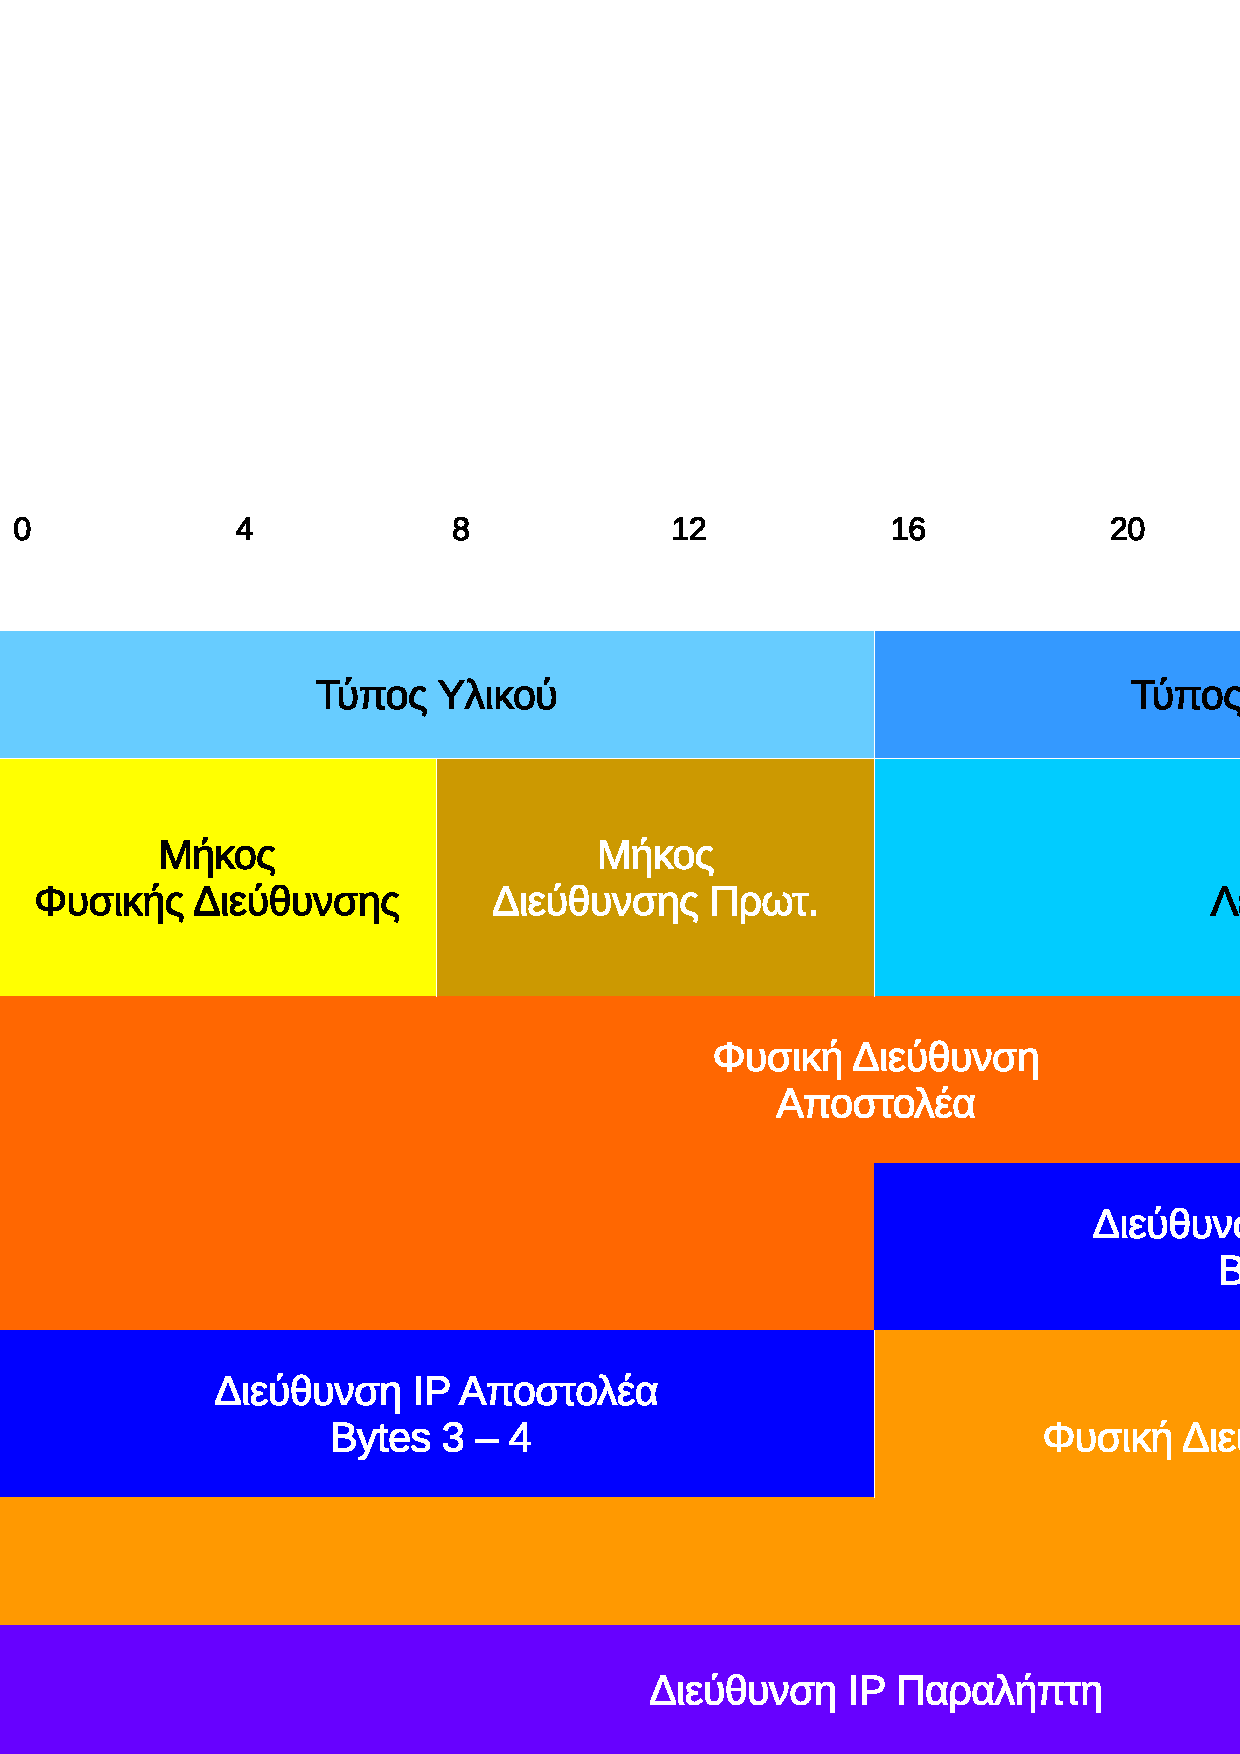
\includegraphics[width=0.85\textwidth]{images/chapter3/3-11}
 \caption {\textsl{Δομή Πακέτου ARP (για Ethernet)}}
 \label{3-11}
\end{figure}

Τα πεδία είναι τα παρακάτω:

\begin{itemize}
\item \textbf{Τύπος Υλικού:} Έχει την τιμή 1 για δίκτυο Ethernet.
\item \textbf{Τύπος Πρωτοκόλλου:} Έχει την τιμή 0x800 (2048) για το IP.
\item \textbf{Μήκος Φυσικής Διεύθυνσης:} Έχει την τιμή 6 για φυσική διεύθυνση Ethernet (έξι bytes).
\item \textbf{Μήκος Διεύθυνσης Πρωτοκόλλου:} Έχει την τιμή 4 για το πρωτόκολλο IPv4 (τέσσερα bytes).
\item \textbf{Κωδικός Λειτουργίας:} Έχει την τιμή 1 για arp request και την τιμή 2 για arp reply.
\end{itemize}

Ακολουθούν οι φυσικές και λογικές διευθύνσεις με τον τρόπο που φαίνεται στο σχήμα (\textbf{Προσοχή:} στο σχήμα του βιβλίου αναγράφεται λανθασμένα η σειρά των bytes της διεύθυνσης πρωτοκόλλου παραλήπτη. Τα δεδομένα τοποθετούνται μέσα στο πλαίσιο ακριβώς όπως θα διαβάζαμε εμείς τη διεύθυνση, κάτι που φαίνεται και στο πρόγραμμα Wireshark).

Στο σχήμα \ref{3-12} φαίνεται το πακέτο arp με κωδικό λειτουργίας 1 (arp request) που αναζητεί τη φυσική διεύθυνση για τον κόμβο με IP 192.168.0.250. Bλέπουμε επίσης και την αντίστοιχη απάντηση (arp reply, με κωδικό λειτουργίας 2).

\begin{figure}[!ht]
 \centering
 \includegraphics[width=0.85\textwidth]{images/chapter3/3-12}
 \includegraphics[width=0.85\textwidth]{images/chapter3/3-13}
 \caption {\textsl{Ερώτημα και Απάντηση ARP}}
 \label{3-12}
\end{figure}

Αν σε μια αναζήτηση φυσικής διεύθυνσης δεν βρεθεί απάντηση στον πίνακα ARP και ούτε δοθεί απάντηση στο ερώτημα ARP, αυτό μπορεί να σημαίνει ότι ο συγκεκριμένος υπολογιστής δεν υπάρχει, είναι σβηστός, ή έχει κάποιο πρόβλημα που τον εμποδίζει να επικοινωνήσει με το δίκτυο. Στην περίπτωση αυτή επιστρέφεται στην εφαρμογή διαγνωστικό μήνυμα που δηλώνει την αδυναμία πρόσβασης. Χαρακτηριστικό παράδειγμα είναι η χρήση της εντολής \emph{ping} σε ανύπαρκτο υπολογιστή:

\begin{center}
\begin{verbatim}
From 10.146.0.110 icmp_seq=3 Destination Host Unreachable
\end{verbatim}
\end{center}

Τα βήματα που ακολουθούνται για την αποστολή ενός πακέτου IP, είναι τα παρακάτω (φαίνονται και στο διάγραμμα ροής στο σχήμα \ref{3-14}):

\begin{figure}[!ht]
 \centering
 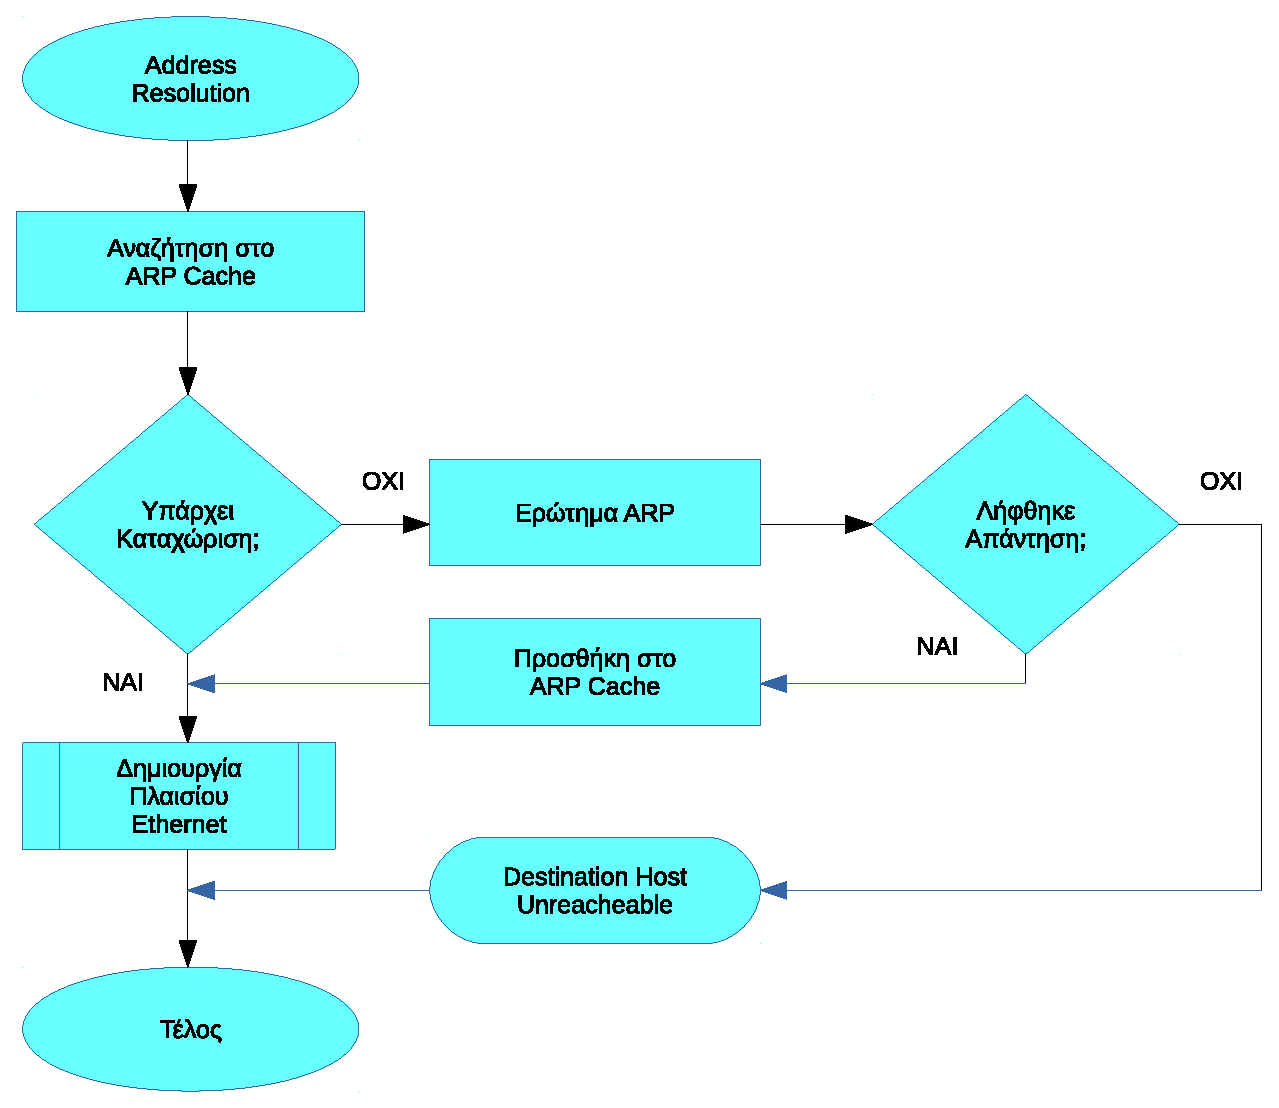
\includegraphics[width=0.85\textwidth]{images/chapter3/3-16}
 \caption {\textsl{Διάγραμμα Ροής για Ανάλυση Διευθύνσεων ARP}}
 \label{3-14}
\end{figure}

\begin{itemize}
\item Το αυτοδύναμο IP πακέτο εισέρχεται στην ουρά αναμονής για μετάδοση.
\item Γίνεται αναζήτηση στον πίνακα ARP για να διαπιστωθεί αν υπάρχει καταχώριση για τη συγκεκριμένη IP.
\item Αν υπάρχει καταχώριση, το πακέτο IP βγαίνει από την ουρά αναμονής, δημιουργείται το αντίστοιχο πλαίσιο Ethernet με βάση την καταχώριση και αποστέλλεται στο δίκτυο.
\item Αν δεν υπάρχει καταχώριση δημιουργείται το κατάλληλο ερώτημα ARP και αποστέλλεται στη διεύθυνση εκπομπής του Ethernet (FF:FF:FF:FF:FF:FF).
\item Αν ληφθεί ARP απάντηση, καταχωρείται στον πίνακα ARP, το πακέτο IP εξέρχεται από την αναμονή, δημιουργείται το αντίστοιχο πλαίσιο Ethernet και αποστέλλεται στο δίκτυο.
\item Αν δεν ληφθεί ARP απάντηση, ο υπολογιστής μπορεί να μην υπάρχει ή να μην είναι ενεργός. Επιστρέφεται στον αποστολέα διαγνωστικό μήνυμα λάθους.
\end{itemize}

Το πρωτόκολλο ARP περιγράφεται στο \href{https://www.ietf.org/rfc/rfc826.txt}{RFC826}.

Εκτός από το πρωτόκολλο ARP, υπάρχει και το πρωτόκολλο \emph{RARP (Reverse Address Resolution Protocol)}. To RARP έχει σκοπό να απλοποιήσει την εγκατάσταση ενός δικτύου: όταν προστίθεται ένας υπολογιστής σε ένα δίκτυο, ο διαχειριστής θα πρέπει να του αποδώσει μια διεύθυνση IP που να συμφωνεί με τις ρυθμίσεις του δικτύου. Ωστόσο θα πρέπει να φροντίσει η διεύθυνση αυτή να είναι μοναδική στο δίκτυο διαφορετικά θα υπάρχει σύγκρουση με κάποιο άλλο υπολογιστή. Σε πολλές περιπτώσεις,είναι προτιμότερο να αποκτά ο υπολογιστής διεύθυνση αυτόματα. Αυτό επιτυγχάνεται με το πρωτόκολλο RARP: στην εκκίνηση, ο υπολογιστής στέλνει ένα κατάλληλα διαμορφωμένο μήνυμα στο δίκτυο και ένας \emph{εξυπηρετητής RARP} αναλαμβάνει να του στείλει κατάλληλη διεύθυνση IP για να χρησιμοποιήσει. Με αυτό τον τρόπο αποφεύγεται η ταλαιπωρία των χειροκίνητων ρυθμίσεων και εξασφαλίζεται ότι δεν θα υπάρχουν συγκρούσεις, αφού ο εξυπηρετητής RARP γνωρίζει ποιες διευθύνσεις έχουν αποδοθεί ήδη και ποιες είναι διαθέσιμες. Το πρωτόκολλο RARP περιγράφεται στο \href{https://www.ietf.org/rfc/rfc903.txt}{RFC903}.

Στις μέρες μας όμως, το RARP χρησιμοποιείται σπάνια, καθώς εκτός από τη διεύθυνση θέλουμε πλέον να στέλνουμε και αρκετές επιπλέον ρυθμίσεις, όπως τη μάσκα δικτύου, την προεπιλεγμένη πύλη, τους διακομιστές DNS κλπ τα οποία το RARP δεν τα καλύπτει. Αντί για το RARP, χρησιμοποιούνται τα πιο σύγχρονα πρωτόκολλα \emph{BOOTP (Bootstrap protocol, πρωτόκολλο εκκίνησης)} και \emph{DHCP, Dynamic Host Configuration Protocol, πρωτόκολλο δυναμικής απόδοσης ρυθμίσεων}.

Το BOOTP προορίζεται κυρίως για χρήση σε υπολογιστές που εκκινούν αποκλειστικά από το δίκτυο και δεν διαθέτουν δικό τους σκληρό δίσκο. Το DHCP είναι πιο ευέλικτο και μπορεί να εξυπηρετήσει τόσο πελάτες BOOTP όσο και μηχανήματα που εκκινούν τοπικά αλλά χρειάζεται να ανακτήσουν τις υπόλοιπες ρυθμίσεις τους από το δίκτυο. Τα δύο αυτά πρωτόκολλο υλοποιούνται στο επίπεδο εφαρμογής, σε αντίθεση με τα ARP/RARP που βρίσκονται στα επίπεδα 2 και 3 του OSI. Είναι εφαρμογές που ακολουθούν το μοντέλο \emph{Πελάτη -- Εξυπηρετητή}.
